\section{Polarization}

\subsection{Capacitance}
The capacitance $C$ is defined by
\begin{equation}
	C = \frac{Q}{V}
\end{equation}
The energy stored in a capacitor is calculated by
\begin{equation}
	E = \frac{1}{2} Q V = \frac{1}{2} C V^2 = \frac{1}{2}\frac{Q^2}{C}
\end{equation}

For a parallel plate capacitor with plate area $A$ and separation $d$, the capacitance is
\begin{equation}
	C = \frac{\varepsilon_0 \varepsilon_r A}{d}
\end{equation}

\subsection{Dipoles}

\begin{figure}[ht]
	\centering
	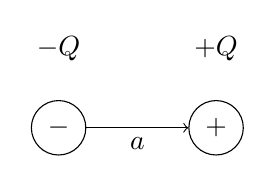
\begin{tikzpicture}
	\node[draw,circle] (qm) at (-1,0) {$-$};
	\node[above of=qm] {$-Q$};
	
	\node[draw,circle] (qp) at (1,0) {$+$};
	\node[above of=qp] {$+Q$};
	
	\draw[->] (qm) to (qp) node[midway, below] {$a$};
\end{tikzpicture}
\end{figure}

The electric dipole moment is
\begin{equation}
	\vec{p} = Q \vec{a}
\end{equation}

When placed in an external electric field $E$, an atom will develop an induced dipole moment
\begin{equation}
	\vec{p}_{\text{induced}} = \alpha \vec{E}
\end{equation}
where $\alpha$ is the electronic polarizability (also $\alpha_e$)

\subsection{Resonance frequency}
To achieve an equilibrium of displacement $x$, the force applied by the electric field $F_e = Ze E$ (where $Z$ is the number of electrons, thus $Z e$ is the displaced charge) has to be equal to the retracting force $F_r = -\beta x$.
Thus $x = \frac{Ze E}{\beta}$. 
The induced el. dipole moment is $p_e = (Ze) x = \frac{(Ze)^2 E}{\beta} = \alpha_e E$.

Assuming a harmonic motion, one finds the differential equation $(Z m_e) \ddot{x} = -\beta\dot{x}$ with the resonance frequency $\omega_0 = \sqrt{\frac{\beta}{Z m_e}}$.

The electronic polarization is then
\begin{equation}
	\alpha_e = \frac{Z^2 e^2}{\beta} = \frac{Z e^2 }{m_e \omega_0^2}
\end{equation}

and the resonance frequency is
\begin{equation}
	\omega_0 = 2 \pi f_0 = \left( \frac{\beta}{Zm_e} \right)^{1/2}
\end{equation}

\subsection{Polarization vector}
The polarization vector $\vec{P}$ is defined as the total dipole moment per unit volume
\begin{equation}
	\vec{P} = N \vec{p}_{av}
\end{equation}
where $N$ is the number of molecules per unit volume and $\vec{p}_{av}$ is the average dipole moment.

For a parallel plate capacitor it follows that
%TODO: add image maybe?
\begin{equation}
	P = \frac{p_{\text{total}}}{\text{volume}} = \frac{Q_P d}{A d} = \frac{Q_P}{A} = \sigma_P
\end{equation}
where$Q_P$ is the positive and negative surface charge ($\pm Q_P$) and $\sigma_P$ is the surface polarization charge density.

The electric susceptility $\chi_e$ is
\begin{equation}
	\chi _e = \frac{1}{\varepsilon_0} N \alpha_e
\end{equation}
From $\vec{D}=\varepsilon_0 \vec{E} + \vec{P} = \varepsilon_0\varepsilon_r \vec{E}$, it follows that
\begin{equation}
	\varepsilon_r  = 1 + \chi_e = 1 + \frac{N \alpha_e}{\varepsilon_0}
\end{equation}

\subsection{Clausius-Mosotti Equation}
The local field in dielectrics is given by
\begin{equation}
	E_{loc} = E + \frac{1}{3 \varepsilon_0} P
\end{equation}

As the local field $E_{loc}$ is larger than the applied field $E$, the Clausius-Mosotti equation is
\begin{equation}
	\frac{\varepsilon_r - 1}{\varepsilon_r+2} = \frac{N \alpha_e}{3 \varepsilon_0}
\end{equation}